\documentclass{article}

\usepackage{arxiv}

\usepackage[utf8]{inputenc} % allow utf-8 input
\usepackage[T1]{fontenc}    % use 8-bit T1 fonts
\usepackage{lmodern}        % https://github.com/rstudio/rticles/issues/343
\usepackage{hyperref}       % hyperlinks
\usepackage{url}            % simple URL typesetting
\usepackage{booktabs}       % professional-quality tables
\usepackage{amsfonts}       % blackboard math symbols
\usepackage{nicefrac}       % compact symbols for 1/2, etc.
\usepackage{microtype}      % microtypography
\usepackage{lipsum}
\usepackage{graphicx}

\title{A linear modelling exploration of predictors of scores in the AFL}

\author{
    Trent Henderson
   \\
    OLET5608 \\
   \\
  \texttt{\href{mailto:then6675@uni.sydney.edu.au}{\nolinkurl{then6675@uni.sydney.edu.au}}} \\
  }


% Pandoc citation processing

\usepackage{amsmath}


\begin{document}
\maketitle

\def\tightlist{}


\begin{abstract}
AFL is a highly-popular Australian sport that has garnered a lot of talk show attention, but suffers from a lack of statistical rigour. The present report seeks to bridge this gap by providing a statistically robust exploration of predictors of scores using data aggregated at the team and match level from the 2005-2019 seasons inclusive. An ordinary least squares regression model was used alongisde preliminary exploration of a more sophisticated generalised additive model approach. Robust variance-covariance matrix estimators were used due to the presence of mild heteroscedasticity. Results found that tackles and unforced errors singificantly and negatively predicted scoring, and rebounds, marks inside 50, marks, inside 50s, handballs, free kicks for, and clearances all significantly and positively predicted scoring. Implications for coaching and gameplay strategy as well as limitations are discussed.
\end{abstract}

\keywords{
    linear modelling, AFL, heteroscedasticity, robust estimation, sports analytics
  }

\hypertarget{introduction}{%
\section{Introduction}\label{introduction}}

AFL is a highly popular Australian sports league that began in 1896 and continues strongly today, with Grand Final match attendance (outside of the anomalous COID-19-impacted 2020 season) approximating a sold out 100,000 each year at the traditional host venue - the Melbourne Cricket Ground (Tables 2021). An AFL match is won based on points, which can be accumulated by kicking either a goal (worth six points) or a behind (worth one point). Despite its popularity and complexity, AFL is a sport that has traditionally relied on subject matter expertise and the knowledge of past players to inform coaching strategies. Much like other Australian sports, a lack of empirical statistical sophistication is evident.

Globally, sports analytics has continued to generate increasing attention, with websites such as FiveThirtyEight and Advanced Sports Analytics creating stylish platforms that constitute a reliable source of insight and interactive analysis. However, this form of innovative and detailed analysis has yet to fully permeate Australian sports. While the AFL has many dedicated talk show analysis television programs such as AFL 360, The Front Bar, and Talking Footy, these programs focus mostly on qualitative breakdowns of high-level descriptive statistics and not on statistical rigour. This report aims to bridge some of this gap by providing a preliminary statistical investigation of factors associated with scoring in the AFL. Specifically, this report aims to explore the following research question: \emph{Which gameplay attributes are predictors of scores in AFL matches?}

\hypertarget{data-set}{%
\section{Data set}\label{data-set}}

Historical AFL data has been made readily-accessible in an open-source setting through the \texttt{R} package \texttt{fitzRoy} (Day, Nguyen, and Lane 2020). The package provides a simple API that accesses and integrates a range of data sources that collate AFL data. Examples of these sources include:

\begin{itemize}
  \item{AFL}
  \item{AFL Tables}
  \item{Squiggle}
  \item{FootyWire}
\end{itemize}

The data itself is diverse, covering domains as broad as player and match statistics, Brownlow medal votes, betting odds, attendance numbers, and match times. This report focuses on player and match statistics by aggregating quantities of interest to team-per-match-level sums using data for the 2005-2019 seasons, inclusive. This time period is somewhat arbitrary, but was made on the basis of wanting a large sample size while balancing recency and homogeneity. The 2020 season is a strong counter example of this, where the season length was truncated and played almost entirely in Queensland due to the impacts of COVID-19. This means the standard set up of games - having a home and away team - was not normal in 2020 and thus data for the entire season may represent a heterogenous set.

\hypertarget{data-limitations}{%
\subsection{Data limitations}\label{data-limitations}}

Despite the availability of so much player-level data, the author of the \texttt{fitzRoy} package and the creators of the sources it pulls from all note potential caveats around their data. The main caveat is that the data is not official. Each source pulls from multiple others, and many individual people are involved in the continual updating of information. The accuracy of the data in \texttt{fitzRoy} is largely contingent on the accuracy of the sources underpinning the websites it scraped. While this is cause for concern, there are a large number of industry-standard sources that comprise the majority of the data used in this report, including official statistics produced by the AFL, newspapers and magazines (such as The Herald Sun and Inside Football), and official books (such as Main and Holmesby (2018) and Rodgers (1996)). The open-source nature of many of the sources, especially AFL Tables, means continual improvement and accuracy is being achieved, further lending confidence to the available data.

\hypertarget{variable-retention}{%
\subsection{Variable retention}\label{variable-retention}}

A small subset of variables were retained from the much larger dataset. The subset was developed based on the author's subject matter expertise of AFL. The variables retained were selected based on their likely relationship to a team's ability to score and whether a team could implement a training or coaching intervention off the back of this analysis to better target important predictors. For example, the variable \emph{free kicks against} was not included, as the number of free kicks given away by a team is not a core contributor to that team scoring, and it is likely near impossible to coach out of their game.

The variables that were retained for the purposes of this analysis included team-match-level counts of scores, marks, handballs, hit outs, tackles, rebounds, inside 50s, clearances, clangers (unforced errors), free kicks for, contested possessions, contested marks, and marks inside 50.

\hypertarget{analysis}{%
\section{Analysis}\label{analysis}}

A rigorous and detailed linear modelling pipeline was implemented. This involved the following steps, each of which will be discussed in turn:

\begin{enumerate}
\def\labelenumi{\arabic{enumi}.}
\tightlist
\item
  Exploratory data analysis and visualisation
\item
  Model fitting and assumption testing
\end{enumerate}

\hypertarget{exploratory-data-analysis-and-visualisation}{%
\subsection{Exploratory data analysis and visualisation}\label{exploratory-data-analysis-and-visualisation}}

Prior to modelling, the data were aggregated and explored visually and numerically to understand the empirical structure. The data was aggregated to match-level sums for each time by summing over individual player statistics. Matches outside of regular season games (i.e.~finals) were removed before any analysis as finals likely represent a heterogenous set. Figure \ref{fig:distplot} shows the distributions of each aggregated quantitative variable.

\begin{figure}
\centering
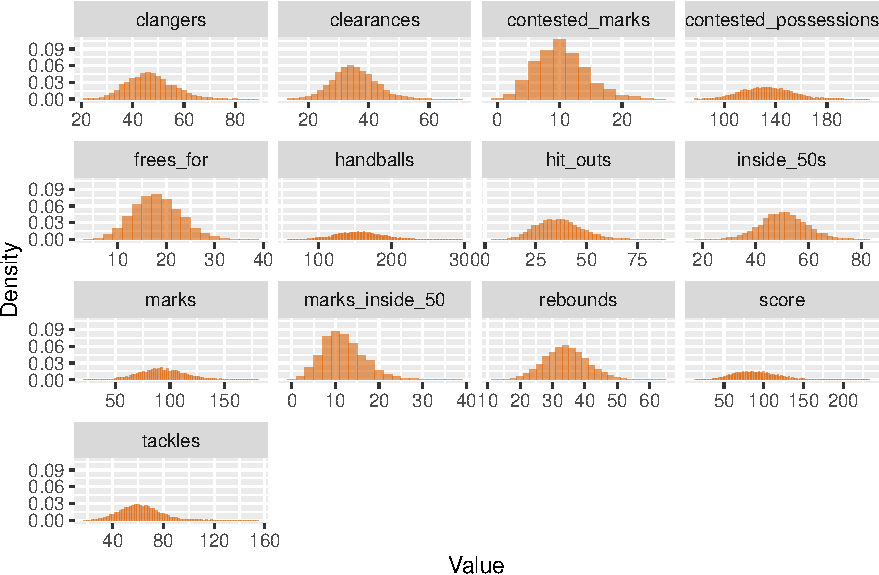
\includegraphics{OLET5608_TrentHenderson_files/figure-latex/distplot-1.pdf}
\caption{\label{fig:distplot}Distribution of raw values for each variable}
\end{figure}

The data were further explored using high-level summary statistics. These are presented in Table \ref{tab:summarystats}. Note the large difference in scales between the variables. To avoid issues with high-variance predictors (due to scale) influencing linear modelling or producing extremely low coefficients, all predictors were mean-centred and standardised (z-scored) prior to modelling. This also means the coefficients will have an intuitive interpretation compared to other rescaling methods.

\begin{table}[ht]
\centering
\begingroup\footnotesize
\begin{tabular}{lrrrrrrrrrr}
 \textbf{Variable} & $\mathbf{n}$ & \textbf{Min} & $\mathbf{q_1}$ & $\mathbf{\widetilde{x}}$ & $\mathbf{\bar{x}}$ & $\mathbf{q_3}$ & \textbf{Max} & $\mathbf{s}$ & \textbf{IQR} & \textbf{\#NA} \\ 
  \hline
score & 5652 & 13 &  70 &  88 &  90.3 & 108 & 233 & 27.9 & 38 & 0 \\ 
  marks & 5652 & 21 &  79 &  93 &  93.5 & 107 & 181 & 21.1 & 28 & 0 \\ 
  handballs & 5652 & 58 & 134 & 155 & 155.5 & 175 & 297 & 30.6 & 41 & 0 \\ 
  hit\_outs & 5652 &  4 &  29 &  36 &  37.2 &  44 &  89 & 11.0 & 15 & 0 \\ 
  tackles & 5652 & 17 &  51 &  61 &  61.6 &  71 & 155 & 15.1 & 20 & 0 \\ 
  rebounds & 5652 & 12 &  30 &  35 &  34.9 &  39 &  65 &  6.9 &  9 & 0 \\ 
  inside\_50s & 5652 & 17 &  45 &  51 &  51.0 &  57 &  83 &  8.5 & 12 & 0 \\ 
  clearances & 5652 & 14 &  31 &  35 &  35.8 &  40 &  71 &  6.9 &  9 & 0 \\ 
  clangers & 5652 & 21 &  41 &  47 &  47.5 &  53 &  89 &  8.8 & 12 & 0 \\ 
  frees\_for & 5652 &  4 &  15 &  18 &  18.6 &  22 &  38 &  4.8 &  7 & 0 \\ 
  contested\_possessions & 5652 & 78 & 120 & 133 & 133.5 & 146 & 213 & 18.7 & 26 & 0 \\ 
  contested\_marks & 5652 &  0 &   8 &  10 &  10.7 &  13 &  27 &  4.0 &  5 & 0 \\ 
  marks\_inside\_50 & 5652 &  0 &   9 &  12 &  12.3 &  15 &  38 &  4.8 &  6 & 0 \\ 
  \end{tabular}
\endgroup
\caption{Descriptive statistics for all quantitative variables} 
\label{tab:summarystats}
\end{table}

\hypertarget{model-fitting-and-assumption-testing}{%
\subsection{Model fitting and assumption testing}\label{model-fitting-and-assumption-testing}}

There are four core assumptions of linear regression model (Faraway 2004). These include:

\begin{enumerate}
\def\labelenumi{\arabic{enumi}.}
\tightlist
\item
  Independent observations
\item
  Linear relationship between \texttt{X} and \texttt{y}
\item
  Normality of residuals
\item
  Homogeneity of variance
\end{enumerate}

Since the data is at the most independent level possible for the present analysis (acknowledging the potential that some relationship may exist between each team on the same match), the following sections will focus on reporting the testing of the other assumptions.

\hypertarget{linear-relationship}{%
\subsubsection{Linear relationship}\label{linear-relationship}}

The purpose of a linear model is to understand the relationship between some number of predictors and a quantitative response variable. As such, a linear model at its core assumes that all predictors are related linearly to the response variable. At this stage, a preliminary linear ordinary least squares (OLS) model was fit which confirmed the visual hypothesis that two variables - \emph{contested marks} and \emph{hit outs} - were not significantly associated with total scores. These variables were dropped for the remaining analysis. Further, as presented in Figure \ref{fig:diagnostics}, a slight quadratic shape is noted on the residuals versus fitted plot at the top left. Three new models were fit in response to this: OLS with second-degree polynomial terms on suspect predictors, OLS with square-root-transformed response, and OLS with log-transformed-response. These models introduced new issues without addressing the underlying problem, and given that the quadratic shape was very slight with the data points themselves looking rather evenly-dispersed, the additional models were not retained.

\begin{figure}
\centering
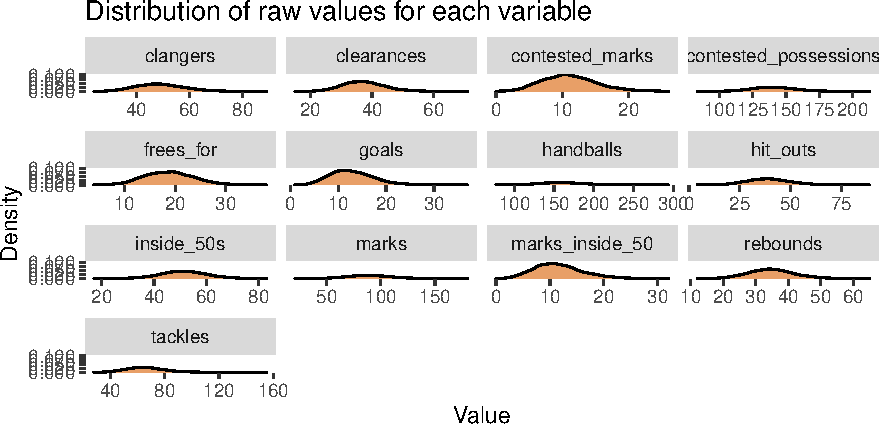
\includegraphics{OLET5608_TrentHenderson_files/figure-latex/unnamed-chunk-4-1.pdf}
\caption{\label{fig:unnamed-chunk-4}Linear relationships between covariates and total score in AFL games}
\end{figure}

While all variables were being tested for appropriateness, a variance inflation factor (VIF) test was undertaken to estimate potential multicollinearity between the predictors. Multicollinearity is an issue as it can drive imprecise estimates, change parameter value signs, and impact \(R^2\) (Hair et al. 2010). Different threshold values exist for VIF, with cutoffs ranging from values less than four being acceptable (Hair et al. 2010) to values less than ten being acceptable (Hair et al. 1995). Outputs from the VIF test are presented below in Table \ref{tab:vif}. Evidently, no predictor violates even the lowest bound commonly cited in the literature, indicating no issue with multicollinearity.

\begin{table}[ht]
\centering
\begin{tabular}{rlrr}
  \hline
 & Variables & Tolerance & VIF \\ 
  \hline
1 & marks & 0.60 & 1.67 \\ 
  2 & handballs & 0.81 & 1.23 \\ 
  3 & tackles & 0.67 & 1.49 \\ 
  4 & rebounds & 0.76 & 1.31 \\ 
  5 & inside\_50s & 0.55 & 1.83 \\ 
  6 & clearances & 0.57 & 1.75 \\ 
  7 & clangers & 0.80 & 1.25 \\ 
  8 & frees\_for & 0.91 & 1.10 \\ 
  9 & contested\_possessions & 0.36 & 2.77 \\ 
  10 & marks\_inside\_50 & 0.59 & 1.68 \\ 
   \hline
\end{tabular}
\caption{Variance inflation factor and tolerance estimates} 
\label{tab:vif}
\end{table}

\hypertarget{normality-of-residuals}{%
\subsubsection{Normality of residuals}\label{normality-of-residuals}}

Normality of residuals is typically assessed graphically using a Q-Q plot, as seen in the upper right graphic in Figure \ref{fig:diagnostics} presented. A model with normally-distributed residuals should lie directly on the diagonal line. The residuals are almost entirely positioned on the line with very little variation at the ends indicating no issues with normality.

\begin{figure}
\centering
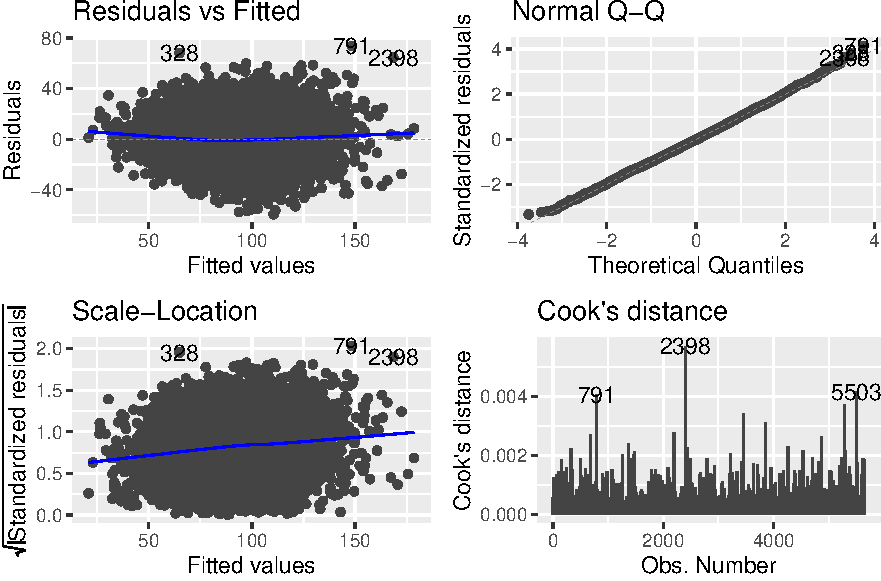
\includegraphics{OLET5608_TrentHenderson_files/figure-latex/diagnostics-1.pdf}
\caption{\label{fig:diagnostics}Linear model diagnostic plots}
\end{figure}

\hypertarget{homogeneity-of-variance}{%
\subsubsection{Homogeneity of variance}\label{homogeneity-of-variance}}

Homoegeneity of variance - the lack of a systematic pattern or bias of residuals across model fitted or predictor values - is another core linear model assumption. This assumption is typically assessed graphically using a residuals and/or standardised plot. A model with homogeneity of variance should have no discernible pattern across the fitted values. This plot is depicted in the bottom left in Figure \ref{fig:diagnostics}.

Evidently, there is a non-horizontal line through the plot, indicating potential heteroscedasticity. Visual inspection of the data points themselves suggests only mild heteroscedasticity as they look reasonably evenly-dispersed. It was first hypothesised that potential outliers might be influencing the results, despite the lack of compelling visual evidence of leverage based on the Cook's distance plot. Following advice from (Faraway 2004), a test of the maximum studentised residual value against a Bonferroni-corrected critical value. Since the maximum residual value of 4.14 was less than the critical value of 4.45, it was declared that outliers were not a major issue.

Heteroscedasticity is a major issue for linear models. As a response to this initial violation, a weighted OLS model was tested The weighted OLS model works by computing weights for each data point included, calculated by the inverse of squared fitted values from a linear regression of the absolute residuals of the original model as the response variable, and the fitted values of the original model as the predictor. The weight vector is then factored into the matrix decomposition to solve the linear regression problem. This method did not fix the heteroscedasticity issue.

As a solution, a heteroscedastic-robust estimator was used, which produces robust estimations of standard errors, test statistics, and \emph{p}-values. This solution may seem like a highly conservative response to the relatively weak violation, however, erring on the side of caution is usually a safe option. Robust estimators are implemented in \texttt{R} using the \texttt{sandwich} package (Zeileis 2004; Zeileis, Köll, and Graham 2020). The estimators work by introducing a new term, \(\Omega\), that flexibly acts on the diagonal of the variance-covariance matrix, and relaxes the assumption of homogeneity by enabling differing variances along the matrix diagonal (see Equation \eqref{eq:vcov} and \eqref{eq:omega}). The inclusion of heteroscedastic-robust estimators reduces the size of test statistics, drives significance values away from zero, and increases standard errors to reflect the variance structure of the data.

\begin{equation}
(X^{'}X)^{-1}X^{'}\Omega X (X^{'}X)^{-1} \label{eq:vcov}
\end{equation}

\begin{equation}
\Omega = \sigma^{2}I_{n} \label{eq:omega}
\end{equation}

Numerous \(\Omega\) options are available in the \texttt{sandwich} package. Most of the options returned negligibly different values for the present analysis, so the default \texttt{HC3} parameter was retained. It is defined according to Equation \eqref{eq:hc3}.

\begin{equation}
HC3 = \frac{\mu^{2}_{\hat{i}}}{(1-h_{i})^{2}} \label{eq:hc3}
\end{equation}

\hypertarget{results}{%
\section{Results}\label{results}}

Coefficients and model outputs are presented in Table \ref{tab:coeftable} where the first column of the dependent variable section is the standard OLS model and the second column is the heteroscedastic-robust correction. Intepretation will focus on the robust estimators, given the violation of homoscedasticity. For each predictor, coefficients, standard errors, \emph{t}-statistics, and \emph{p}-values are reported. Since all predictors were mean-centred and standardised (z-scored) prior to analysis, the interpretation is as follows: \emph{the coefficient represents the expected change in total score (response variable) for a one standard deviation change in the predictor}. The overall model is statistically significant, \emph{F} = 811.8 (\emph{df} = 10; 5641), and explains approximately 59\% of the observed variance in scores.

Two predictors were negative and statistically significant. These were tackles (\emph{t} = -4.28, \emph{p} \textless{} .001) and clangers (\emph{t} = -15.54, \emph{p} \textless{} .001), such that a one standard deviation increase in tackles is associated with mean reduction of 1.2 in total score, and a one standard deviation increase in clangers is associated with mean reduction of 4.2 in total score. For the positive predictors, the two with the strongest coefficients are mechanically related in terms of AFL gameplay: inside 50s (\emph{t} = 28.03, \emph{p} \textless{} .001) and marks inside 50 (\emph{t} = 38.6, \emph{p} \textless{} .001). The magnitude of both these predictors is noteworthy, as a one standard deviation increase in inside 50s is associated with a mean increase of 9.3 in total score, and a one standard deviation increase in marks inside 50 is associated with a mean increase of 12.2 in total score. The remaining positive predictors are presented in Table \ref{tab:coeftable} below.

\begin{table}[!htbp] \centering 
  \caption{Model coefficients, confidence intervals, and signifiance tests} 
  \label{tab:coeftable} 
\begin{tabular}{@{\extracolsep{5pt}}lcc} 
\\[-1.8ex]\hline 
\hline \\[-1.8ex] 
 & \multicolumn{2}{c}{\textit{Dependent variable:}} \\ 
\cline{2-3} 
\\[-1.8ex] & score &   \\ 
\\[-1.8ex] & \textit{OLS} & \textit{coefficient} \\ 
 & \textit{} & \textit{test} \\ 
\\[-1.8ex] & (1) & (2)\\ 
\hline \\[-1.8ex] 
 marks & 2.321 (1.720, 2.922) & 2.321 (1.721, 2.921) \\ 
  & t = 7.570$^{***}$ & t = 7.583$^{***}$ \\ 
  & p = 0.000 & p = 0.000 \\ 
  handballs & 1.198 (0.681, 1.714) & 1.198 (0.676, 1.719) \\ 
  & t = 4.541$^{***}$ & t = 4.502$^{***}$ \\ 
  & p = 0.00001 & p = 0.00001 \\ 
  tackles & $-$1.224 ($-$1.793, $-$0.656) & $-$1.224 ($-$1.785, $-$0.663) \\ 
  & t = $-$4.221$^{***}$ & t = $-$4.276$^{***}$ \\ 
  & p = 0.00003 & p = 0.00002 \\ 
  rebounds & 0.980 (0.448, 1.513) & 0.980 (0.440, 1.521) \\ 
  & t = 3.609$^{***}$ & t = 3.557$^{***}$ \\ 
  & p = 0.0004 & p = 0.0004 \\ 
  inside\_50s & 9.317 (8.687, 9.947) & 9.317 (8.666, 9.969) \\ 
  & t = 28.974$^{***}$ & t = 28.029$^{***}$ \\ 
  & p = 0.000 & p = 0.000 \\ 
  clearances & 4.198 (3.582, 4.815) & 4.198 (3.562, 4.835) \\ 
  & t = 13.348$^{***}$ & t = 12.930$^{***}$ \\ 
  & p = 0.000 & p = 0.000 \\ 
  clangers & $-$4.163 ($-$4.684, $-$3.642) & $-$4.163 ($-$4.688, $-$3.638) \\ 
  & t = $-$15.667$^{***}$ & t = $-$15.542$^{***}$ \\ 
  & p = 0.000 & p = 0.000 \\ 
  frees\_for & 2.015 (1.528, 2.503) & 2.015 (1.526, 2.505) \\ 
  & t = 8.102$^{***}$ & t = 8.071$^{***}$ \\ 
  & p = 0.000 & p = 0.000 \\ 
  contested\_possessions & 1.009 (0.233, 1.784) & 1.009 (0.208, 1.810) \\ 
  & t = 2.550$^{*}$ & t = 2.469$^{*}$ \\ 
  & p = 0.011 & p = 0.014 \\ 
  marks\_inside\_50 & 12.202 (11.598, 12.806) & 12.202 (11.583, 12.822) \\ 
  & t = 39.599$^{***}$ & t = 38.618$^{***}$ \\ 
  & p = 0.000 & p = 0.000 \\ 
  Constant & 90.267 (89.802, 90.733) & 90.267 (89.801, 90.733) \\ 
  & t = 380.134$^{***}$ & t = 379.740$^{***}$ \\ 
  & p = 0.000 & p = 0.000 \\ 
 \hline \\[-1.8ex] 
Observations & 5,652 &  \\ 
R$^{2}$ & 0.590 &  \\ 
Adjusted R$^{2}$ & 0.589 &  \\ 
Residual Std. Error & 17.852 (df = 5641) &  \\ 
F Statistic & 811.824$^{***}$ (df = 10; 5641) &  \\ 
\hline 
\hline \\[-1.8ex] 
\textit{Note:}  & \multicolumn{2}{r}{$^{*}$p$<$0.05; $^{**}$p$<$0.01; $^{***}$p$<$0.001} \\ 
\end{tabular} 
\end{table}

\hypertarget{discussion}{%
\section{Discussion}\label{discussion}}

The present analysis aimed to produce an innovative and statistically robust exploration of predictors of scoring in the AFL using team-per-match-level data for the 2005-2019 seasons inclusive accessed through the \texttt{R} package \texttt{fitzRoy}. While not necessarily causal, the analysis sought to quantify the type and magnitude of any relationships with end-of-match scores.

\hypertarget{implications-for-afl-teams}{%
\subsection{Implications for AFL teams}\label{implications-for-afl-teams}}

This report found some potentially informative relationships regarding scoring in the AFL that teams may seek to consider. First, teams should seek to deeply understand their potential to generate opportunities within the fifty-metre circle in front of goal. The analysis strongly supports this recommendation, as increases in inside 50s and marks inside 50 is associated with a very substantial increase in total score. From a gameplay sense this is intuitive, as being closer to goal with possession of the ball would increase the likelihood of scoring, and a mark inside 50 means a guaranteed uninterrupted set shot at goal, further increasingly the likelihood of kicking a six-point goal.

Second, teams should also consider the importance of clearances. The strong positive association found between clearances and scores was surprising. This is because clearances involve a team kicking the ball away from their own goal area, which is a heavily defensive statistic. The positive relationship may suggest that the opposition team was unsuccessful in scoring on multiple occasions, and so the team could take advantage of converting a successful defense into attacking opportunities of their own.

Third, teams should be cautious not to interpret the causal direction of some of the relationships presented in this report. The negative relationship between tackles and scores is one such example. It is not necessarily the case that tackling less directly results in higher scores at the end of a match. It is far more likely that teams who score more (therefore more likely winning more) are just more defensively efficient or spend more time attacking rather than defending. Both of these characteristics would manifest as noticeably lower tackle counts.

\hypertarget{limitations}{%
\subsection{Limitations}\label{limitations}}

Despite the potentially informative findings, there were some limitations with the analysis. The first, as described earlier, is that the data is not official, and therefore its accuracy is unknown. It is likely that the data quality is high, given that some of the underlying sources are official and published material and that the project is open-source with contributions for numerous high-profile researchers and analysts.

A second limitation is that of variable selection. The variables included in this analysis were selected based on the author's subject matter expertise and prior knowledge of AFL. However, these variables only explained roughly sixty per cent of the variance in match scores. It is highly likely that the addition of more variables included in the larger dataset of approximately sixty variables would help drive this number closer to a more respectable percentage, such as eighty or ninety per cent. Since factor variables are included in the broader dataset, their inclusion raises some interesting questions around interaction terms. For example, future research may seek to fit interaction terms by team, or by home versus away, to better understand the dynamics of AFL metrics on match scores. Of course, the inclusion of more covariates, especially large numbers of them, may raise serious issues around multicollinearity or other model assumptions. Researchers may seek to account for this by first applying variable selection procedures such as Lasso regression (Tibshirani 1996).

A third limitation is that of model selection. It remains unclear whether an ordinary least squares regression approach is the optimal modelling technique for this data. Preliminary follow-up analysis undertaken by the author revealed that a generalised additive model (Hastie and Tibshirani 1986; Wood, n.d., 2011) - a model that linearly adds estimated smooth functions using splines for each covariate - produced a better model fit at a lower Akaike information criterion value (Posada and Buckley 2004). Further, since the response variable is a non-zero count, it may be more appropriate to consider a generalised linear model with a link function appropriate to an integer response, such as a Poisson or negative binomial-distributed model. The added benefit of these models is that they correctly model the response as a discrete-valued probability mass function, instead of the probability density function assumed by a Gaussian linear model (if a maximum likelihood and not ordinary least squares approach is taken). This may be particularly pertinent if future endeavours focus on predictive applications. Future research should aim to consider these modelling options, and potentially even perform a direct comparison.

\hypertarget{available-code}{%
\section{Available code}\label{available-code}}

All code for this report is available on \href{https://github.com/hendersontrent/phd-coursework/tree/main/olet5608}{GitHub}.

\pagebreak

\hypertarget{references}{%
\section*{References}\label{references}}
\addcontentsline{toc}{section}{References}

\hypertarget{refs}{}
\leavevmode\hypertarget{ref-fitzRoy}{}%
Day, James, Robert Nguyen, and Oscar Lane. 2020. \emph{FitzRoy: Easily Scrape and Process Afl Data}. \url{https://CRAN.R-project.org/package=fitzRoy}.

\leavevmode\hypertarget{ref-R:Faraway:2004}{}%
Faraway, Julian J. 2004. \emph{Linear Models with R}. Chapman \& Hall/CRC. \url{http://www.maths.bath.ac.uk/\%20jjf23/LMR/}.

\leavevmode\hypertarget{ref-multi2}{}%
Hair, J. F., R. E. Anderson, R. L. Tatham, and W. C. Black. 1995. \emph{Multivariate Data Analysis (3rd Ed.)}. Macmillan Publishing Company, New York.

\leavevmode\hypertarget{ref-multi1}{}%
Hair, J. F., W. C. Black, B. J. Babin, and R. E. Anderson. 2010. \emph{Multivariate Data Analysis (7th Ed.)}. Upper saddle River, New Jersey: Pearson Education International.

\leavevmode\hypertarget{ref-10.1214ux2fssux2f1177013604}{}%
Hastie, Trevor, and Robert Tibshirani. 1986. ``Generalized Additive Models.'' \emph{Statistical Science} 1 (3): 297--310. \url{https://doi.org/10.1214/ss/1177013604}.

\leavevmode\hypertarget{ref-everyone}{}%
Main, Jim, and Russel Holmesby. 2018. \emph{The Encyclopedia of Afl Footballers: Every Afl/Vfl Player Since 1897}. Bas Publishing.

\leavevmode\hypertarget{ref-10.1080ux2f10635150490522304}{}%
Posada, David, and Thomas R. Buckley. 2004. ``Model Selection and Model Averaging in Phylogenetics: Advantages of Akaike Information Criterion and Bayesian Approaches Over Likelihood Ratio Tests.'' \emph{Systematic Biology} 53 (5): 793--808. \url{https://doi.org/10.1080/10635150490522304}.

\leavevmode\hypertarget{ref-everygame}{}%
Rodgers, Stephen. 1996. \emph{Every Game Ever Played: VFL/Afl Results, 1897-1995}. Viking.

\leavevmode\hypertarget{ref-attendance}{}%
Tables, AFL. 2021. ``Grand Finals.'' \url{https://afltables.com/afl/teams/allteams/gfgames.html}.

\leavevmode\hypertarget{ref-https:ux2fux2fdoi.orgux2f10.1111ux2fj.2517-6161.1996.tb02080.x}{}%
Tibshirani, Robert. 1996. ``Regression Shrinkage and Selection via the Lasso.'' \emph{Journal of the Royal Statistical Society: Series B (Methodological)} 58 (1): 267--88. \url{https://doi.org/https://doi.org/10.1111/j.2517-6161.1996.tb02080.x}.

\leavevmode\hypertarget{ref-mgcv}{}%
Wood, S. N. 2011. ``Fast Stable Restricted Maximum Likelihood and Marginal Likelihood Estimation of Semiparametric Generalized Linear Models.'' \emph{Journal of the Royal Statistical Society (B)} 73 (1): 3--36.

\leavevmode\hypertarget{ref-wood}{}%
---------. n.d. ``Frequently Asked Questions for Package Mgcv.'' \url{http://web.mit.edu/~r/current/arch/i386_linux26/lib/R/library/mgcv/html/mgcv-FAQ.html}.

\leavevmode\hypertarget{ref-JSSv011i10}{}%
Zeileis, Achim. 2004. ``Econometric Computing with Hc and Hac Covariance Matrix Estimators.'' \emph{Journal of Statistical Software, Articles} 11 (10): 1--17. \url{https://doi.org/10.18637/jss.v011.i10}.

\leavevmode\hypertarget{ref-JSSv095i01}{}%
Zeileis, Achim, Susanne Köll, and Nathaniel Graham. 2020. ``Various Versatile Variances: An Object-Oriented Implementation of Clustered Covariances in R.'' \emph{Journal of Statistical Software, Articles} 95 (1): 1--36. \url{https://doi.org/10.18637/jss.v095.i01}.

\bibliographystyle{unsrt}
\bibliography{references.bib}


\end{document}
